% ------------------------------------------------------------------------
% file `v3-exercise-4-solution-body.tex'
%   in folder `xsim/'
%
%     solution of type `exercise' with id `4'
%
% generated by the `solution' environment of the
%   `xsim' package v0.20c (2021/02/03)
% from source `v3' on 2022/06/03 on line 135
% ------------------------------------------------------------------------
    1 point par bonne réponse.
    2 point pour le tableau de signe.
    2 point pour le tableau de variation.
    -1 point par erreur dans les tableaux de signes et de variations.
    \begin{tasks}(2)
        \task $\textrm{dom }f=[-9,-6[~\cup~[-5,3[$
        \task $\textrm{im }f=[-2,3]$
        \task $-2$
        \task $\lbrace -7;-2;2 \rbrace$
        \task!
        \begin{tikzpicture}[baseline=(current bounding box.north)]
            \tkzTabInit[espcl=1.5]%
            {$x$/1, $f(x)$/1}%
            {$-9$,$-7$,$-6$,$-5$,$-2$,$2$,$3$}
            \tkzTabLine{-,-,z,+,d,h,+,+,z,-,z,+,d}
        \end{tikzpicture}
        \task!
        \begin{tikzpicture}[baseline=(current bounding box.north)]
            \tkzTabInit[espcl=1.5]%
            {$x$/1, $f(x)$/1.5}%
            {$-9$,$-6$,$-5$,$0$,$3$}
            \tkzTabVar{-/$-2$,+DH/,+/$3$,-/$-2$,+D/}
        \end{tikzpicture}
        \task $1$
        \task $2$
    \end{tasks}
